\documentclass[margin=1mm]{standalone}
\usepackage{enumitem}
\usepackage[skip=3mm, indent=0mm]{parskip}
\usepackage{fontspec}
\setmainfont{QTHeidelbergType}

\usepackage[x11names]{xcolor}
\usepackage{tikz}
\colorlet{fascist}{OrangeRed1}
\colorlet{liberal}{Turquoise4}

\begin{document}
	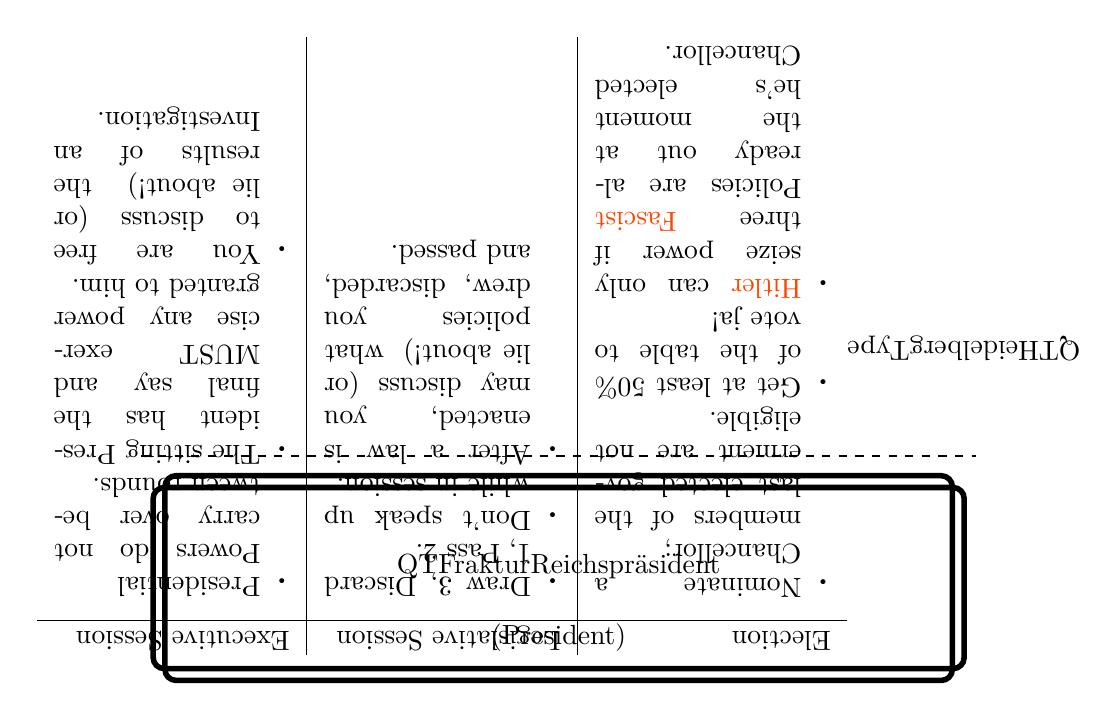
\begin{tikzpicture}		
		
		\node at (0,0) {\fontsize{40}{40}\setmainfont{QTFraktur}Reichspräsident};
		\node at (0,-0.9) {(President)};
		
		\draw [line width=2, rounded corners] (-5.15,1) rectangle (5.15,-1.3);
		\draw [line width=2, rounded corners] (-5,1.15) rectangle (5,-1.45);
		
		\fill [white] (-5.3, 1.4) rectangle (5.3, 4.25);
		\draw [dashed, line width=1] (-5.3, 1.4)--(5.3, 1.4);
		%\draw (-5.3, 1.7) rectangle (5.3, 4);
		
		\begin{scope}[yshift=2.8cm]
			\node at (0,0) [rotate=180] {\fontsize{6}{6}\setmainfont{QTHeidelbergType}\begin{tabular}{p{3cm}|p{3cm}|p{3cm}}
				Election & Legislative Session & Executive Session\\
				\hline
				\begin{itemize}[leftmargin=*]
					\item Nominate a Chancellor; members of the last elected goverment are not eligible.
					\item Get at least 50\% of the table to vote ja!
					\item \textcolor{fascist}{Hitler} can only seize power if three \textcolor{fascist}{Fascist} Policies are already out at the moment he's elected Chancellor.
				\end{itemize} & 
				\begin{itemize}[leftmargin=*]
					\item Draw 3, Discard 1, Pass 2.
					\item Don't speak up while in session.
					\item After a law is enacted, you may discuss (or lie about!) what policies you drew, discarded, and passed.
				\end{itemize} & 
				\begin{itemize}[leftmargin=*]
					\item Presidential Powers do not carry over between rounds.
					\item The sitting President has the final say and MUST exercise any power granted to him.
					\item You are free to discuss (or lie about!) the results of an Investigation.
				\end{itemize} 
			\end{tabular}};
		\end{scope}
		
	\end{tikzpicture}
\end{document}